\toggletrue{image}
\toggletrue{imagehover}
\chapterimage{tall_infographics_2x}
\chapterimagetitle{\uppercase{Tall Infographics}}
\chapterimageurl{https://xkcd.com/1273/}
\chapterimagehover{'Big Data' doesn't just mean increasing the font size.}

%https://cgvr.informatik.uni-bremen.de/teaching/info1_0506/folien/02_repraesentation_daten_2up_1.pdf
%https://files.ifi.uzh.ch/ee/fileadmin/user_upload/teaching/hs12/02_FGI_Information_Text.pdf

\chapter{Information}
\label{chapter-information}

In diesem Kapitel klären wir, was man unter dem Begriff Information versteht. Die Lernziele lauten:

\newcommand{\informationLernziele}{
\protect\begin{todolist}
\item Sie definieren den Begriff Information.
\item Sie nennen ein Beispiel für eine Information.
\end{todolist}
}

\lernziel{\autoref{chapter-information}, \nameref{chapter-information}}{\protect\informationLernziele}

\informationLernziele

\section{Was ist Information?}

Menschen interessieren sich für Informationen und führen eine Informationsverarbeitung durch. Auch die Informatik beschäftigt sich mit Information. Dies haben wir bereits in der Begriffsdefinition aus \autoref{chapter-was-ist-informatik} gesehen. Auch das Wort selbst (Informatik) entstand (vermutlich) aus der Modifikation des Wortes Information. Was verstehen wir eigentlich unter Information? Es ist ein abstrakter Begriff, der zahlreiche Definitionen hat und schlecht greifbar ist. Wir einigen uns auf folgende Definition.

\begin{definition}[Information]
	Eine Information sind Daten mit einer Bedeutung. Dies kann ein gesprochener oder geschriebener Text sein, ein Bild, ein Geräusch, ein Duft oder eine Empfindung sein. Wir können diese Informationen mit unseren Sinnesorganen wahrnehmen und durch technische Hilfsmittel speichern oder übertragen.
\end{definition}

\begin{example} Der Satz \say{The quick brown fox jumps over the lazy dog.} stellt eine Information dar oder der Fahrplan an einer Bushaltestelle. Auch das Bild aus \autoref{figure-portland} ist eine Information. Die Bedeutung einer Information ist subjektiv. Für Personen, welche kein klingonisch können, ist das Wort jI-yaj-be bedeutungslos.

\begin{figure}[htb]
\centering
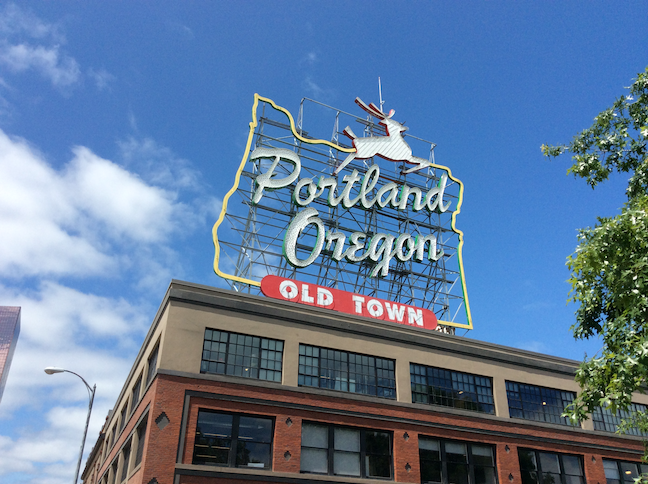
\includegraphics[scale=0.25]{portland.png}
\caption{Portland (USA).}
\label{figure-portland}
\end{figure}

\end{example}